\documentclass[10pt, conference]{IEEEtran}

\usepackage{cite}
\usepackage{amsmath,amssymb,amsfonts}
\usepackage{algorithmic}
\usepackage{textcomp}
\usepackage{booktabs}
\usepackage{listings}
\usepackage{multirow}
\usepackage{graphicx}
\usepackage{subcaption}
\usepackage[hidelinks]{hyperref}
\usepackage{fancybox}
\usepackage{enumitem}
\usepackage{xcolor}
\usepackage[export]{adjustbox}
\usepackage{xspace}
\def\BibTeX{{\rm B\kern-.05em{\sc i\kern-.025em b}\kern-.08em
    T\kern-.1667em\lower.7ex\hbox{E}\kern-.125em X}}


\definecolor{listinggray}{gray}{0.9}
\definecolor{lbcolor}{rgb}{0.9,0.9,0.9}
\definecolor{dkgreen}{rgb}{0,0.5,0}
\definecolor{dkred}{rgb}{0.5,0,0}
\definecolor{gray}{rgb}{0.5,0.5,0.5}
\definecolor{cyan(process)}{rgb}{0.0, 0.72, 0.92}
\definecolor{safetyorange}{rgb}{1.0, 0.4, 0.0}
\definecolor{javagreen}{rgb}{0.25,0.5,0.35}
\definecolor{metalgrey}{rgb}{0.43, 0.5, 0.5}
 % comments
%basicstyle=\ttfamily\bfseries\footnotesize,


\lstdefinestyle{JavaStyle}{
    language=Java,      % choose the language of the code
    keywords=[2]{View, LayoutInflater, ViewGroup, Bundle, ListView, Fragment, Activity},
    keywords=[3]{onCreateView, inflate, getActivity, DLE, findViewById, setAdapter},
    keywords=[4]{@Override, listView, DirList},
    basicstyle=\ttfamily\bfseries,
    keywordstyle=\color[RGB]{69,97,189},
    keywordstyle=[2]{\color{cyan(process)}},
    keywordstyle=[3]\color{javagreen},
    keywordstyle=[4]\color{metalgrey},
    %safetyorange
    commentstyle=\itshape\color{green!60!black},
    moredelim=[l][\itshape\color{gray}]{//}, %<--- overrides line-comment style
    stringstyle=\color[RGB]{192,8,8},
    numberstyle=\itshape\color{yellow!50!black},
%   backgroundcolor=\color{lbcolor},
    tabsize=4,
%   rulecolor=,
    upquote=true,
    aboveskip={1.5\baselineskip},
    columns=fixed,
    showstringspaces=false,
    extendedchars=false,
    breaklines=true,
    prebreak = \raisebox{0ex}[0ex][0ex]{\ensuremath{\hookleftarrow}},
    frame=single,
    numbers=left,
    showtabs=false,
    showspaces=false,
    showstringspaces=false,
    %autodedent,%<--- removes indentation
}
\lstdefinestyle{examplestyle}{
    language=C,      % choose the language of the code
    basicstyle=\ttfamily\footnotesize\bfseries,
    tabsize=4,
    aboveskip={.25\baselineskip},
    belowskip={.25\baselineskip},
    columns=fixed,
    showstringspaces=false,
    extendedchars=false,
    breaklines=true,
    prebreak = \raisebox{0ex}[0ex][0ex]{\ensuremath{\hookleftarrow}},
    frame=none,
    numbers=none,
    showtabs=false,
    showspaces=false,
    showstringspaces=false,
    %autodedent,%<--- removes indentation
}

\lstset{style=JavaStyle}

\newcommand\todo[1]{\textcolor{red}{#1}}
\newcommand\bears{\textsc{Bears}\xspace}

\begin{document}

\title{A Study of Multi-Location Bug Patches}

\author{Anonymous Authors}

%% JL: This is the author template from the IEEE example tex file.
%%
%% \author{\IEEEauthorblockN{1\textsuperscript{st} Given Name Surname}
%% \IEEEauthorblockA{\textit{dept. name of organization (of Aff.)} \\
%% \textit{name of organization (of Aff.)}\\
%% City, Country \\
%% email address or ORCID}
%% \and
%% \IEEEauthorblockN{2\textsuperscript{nd} Given Name Surname}
%% \IEEEauthorblockA{\textit{dept. name of organization (of Aff.)} \\
%% \textit{name of organization (of Aff.)}\\
%% City, Country \\
%% email address or ORCID}
%% \and
%% \IEEEauthorblockN{3\textsuperscript{rd} Given Name Surname}
%% \IEEEauthorblockA{\textit{dept. name of organization (of Aff.)} \\
%% \textit{name of organization (of Aff.)}\\
%% City, Country \\
%% email address or ORCID}
%% \and
%% \IEEEauthorblockN{4\textsuperscript{th} Given Name Surname}
%% \IEEEauthorblockA{\textit{dept. name of organization (of Aff.)} \\
%% \textit{name of organization (of Aff.)}\\
%% City, Country \\
%% email address or ORCID}
%% \and
%% \IEEEauthorblockN{5\textsuperscript{th} Given Name Surname}
%% \IEEEauthorblockA{\textit{dept. name of organization (of Aff.)} \\
%% \textit{name of organization (of Aff.)}\\
%% City, Country \\
%% email address or ORCID}
%% \and
%% \IEEEauthorblockN{6\textsuperscript{th} Given Name Surname}
%% \IEEEauthorblockA{\textit{dept. name of organization (of Aff.)} \\
%% \textit{name of organization (of Aff.)}\\
%% City, Country \\
%% email address or ORCID}
%% }

\maketitle

\begin{abstract}
    Automatic program repair is a promising approach for reducing the
    cost of quality assurance practices and faulty software. To date, most
    techniques proposed for test-driven automatic repair succeed
    primarily on bugs that benefit from short, single-location patches. Techniques
    that successfully generate multi-location patches often do so in an
    alternative, single-edit way, or by targeting particular multi-location bug
    patterns. Empirical studies of real-world bugs similarly tend to focus on the
    patterns exhibited by single-location bug patches, and have not examined repairability
    of multi-location patches in detail. We present a comprehensive empirical analysis
    of multi-location patches for bugs in open source Java programs, focusing on static and
    dynamic properties that define the repair search space for a given bug.
    This analysis focuses on key challenges of the dynamic program repair
    problem: the \emph{mutations and fix code} used to repair bugs in multiple locations;
    the \emph{fault locations} and their relationships; and the \emph{evaluation},
    and in particular how and to what degree tests can be used
    (or not) to identify partial repairs. We identify key takeaways and
    challenges, with implications for future work in expressive, multi-location bug
    repair.
\end{abstract}

\begin{IEEEkeywords}
  software bugs, program repair
\end{IEEEkeywords}

\newcommand{\rqorinsight}[2]{
  \setlength{\fboxsep}{0.8em}
  \vspace{-0.5em}
  \begin{center}
  \Ovalbox{\begin{minipage}{0.95\linewidth}
    \textbf{RQ#1:} #2
    \end{minipage}}
  \end{center}
  \vspace{0.5em}
}

\section{Introduction}

\renewcommand\todo[1]{}

Buggy software has a significant economic cost~\cite{cambridge-study}, and
software failures are estimated to have affected half of the world's
population~\cite{tricentis}.  This motivates research in
techniques to automatically find and fix bugs, some of which
began to be integrated into
real-world development practices~\cite{iceland,sapfix,getafix}.

A significant class of program repair techniques in both
research~\cite{genprog,angelix,Le17,Xuan17,arja-journal,prapr,saha2019harnessing,astor}
and practice~\cite{sapfix} use test
cases to guide patch construction. At a high level, these techniques use test cases
to localize a defect --- identified by at least one failing test --- and to
validate which (if any) of the generated patch candidates lead
the program to pass all tests.
Patches are constructed in a variety of ways, ranging from heuristic, syntactic
program manipulation~\cite{par,genprog,rsrepair,ae,prophet,hdrepair,arja-journal,confix,saha2019harnessing},
to specially adapted program synthesis 
techniques~\cite{Konighofer11,Konighofer12,semfix,DeMarco14,angelix,sosrepair,Xuan17}. 
These techniques have successfully
repaired meaningful defects in complex
programs~\cite{angelix,genprog-eight-dollars,sapfix,durieux-repair-them-all}.

Practically speaking, though, these techniques are typically limited in the types and
complexity of defects they can repair. Often this is by design: techniques may
limit the repair search space to single-location patches for
tractability~\cite{rsrepair,ae,hdrepair,capgen}, while others only target certain
classes of bugs~\cite{Xuan17,sapfix,DeMarco14,par}. However, even techniques
that can in principle generate repairs with multi-location patches typically
don't~\cite{patch-correctness}.
%
Meanwhile, many real-world bugs require multi-location 
patches~\cite{d4j-dissection,zhong2015}, leaving a large
proportion of them unrepairable by modern
research techniques in program repair.  
%Over half of the bugs in the popular bug
%benchmark Defects4J are patched by humans using multi-part
%patches~\cite{d4j-dissection}. Approximately 70\% of buggy source files in a
%large study of bugs in Apache projects required edits at two or more
%locations~\cite{zhong2015}.

This is a difficult problem.
A key tension in the design of an automated repair technique is the balance
between giving users confidence in patch correctness by maximizing its
subjective quality while managing a trivially-infinite search space. This space
is typically parameterized along several axes: (1) the \emph{fault space}:
potential program locations to be modified, (2) the \emph{mutation space}: which
modifications may be applied at a location, and (3) the \emph{fix space}: code
that may be instantiated for a specific mutation. For example, a repair
technique might identify the location of a null-pointer dereference (exploring
the fault space), decide to insert new code (mutation space), and synthesize
code to initialize the pointer (fix space). 

Multi-location repair poses distinct challenges for each of these repair axes.
Spectrum-based fault localization~\cite{ochiai}, the most prevalent class of
fault localization used in program repair, does not specifically
identify sets of potentially-related locations; indeed,
the evaluation of most fault localization techniques typically assumes that a bug
is localized if any one buggy line is identified~\cite{fl-survey-wong}.
Some bugs \emph{are}
repaired in multiple locations using very similar
code~\cite{saha2019harnessing,jiang2019cmsuggester}, informing novel techniques
that constrain the \emph{fix space} of possible multi-location repairs accordingly.
But, how prevalent are these bugs, 
relative to those that require multiple
coordinating edits?
Note for example that over 50\% of the fixes in four 
Apache projects involve two or more  Java classes, methods, or fields, and  66\%-76\% of 
those multi-entity fixes involved syntactic dependencies~\cite{wang2018}. 
Test cases are used to evaluate candidate repairs in dynamic
repair techniques, but may not be effective
at identifying partial repairs in a multi-location
context~\cite{better-fitness}.  
Although multi-location repair has been discussed in the context of other analyses
that study bug fix characteristics in general~\cite{d4j-dissection} as well as for
repair applicability specifically~\cite{zhong2015, wang2018}, 
% Do Motwani et al study this?
to our
knowledge there has been no previous significant study of the characteristics of
multi-location repairs and their implications for automatic
repair.

To lay groundwork for more informed, systematic research
efforts in the space of multi-edit repair, we conduct a systematic study of real-world bugs with
multi-location patches.  We study bugs curated in two
real-world datasets that support program repair research: Defects4J~\cite{defects4j}
and \bears~\cite{bears}, in total, 1018 bugs in 51 projects.
More than half of these bugs were repaired by a
human developer using edits at multiple locations.  We look at characteristics along each of the
relevant axes of the program repair search problem: fault locations, mutation
operators, fix code, and evaluation (or fitness or objective) using test cases,
and find both important and, in some cases, unintuitive, implications for
APR.  Our contributions are:

\begin{itemize}
%\item An analysis and enumeration of multi-location patches in Defects4J and
%\bears.
% I think the above is addressed by the summary in the preceding paragraph.
\item \textbf{Fault Localization.}  We find that 67\% of multi-location bugs have faulty 
locations that are not
  covered by all failing tests.  This is important because this violates an assumption underlying 
  spectrum-based
  fault localization. Thus, off-the-shelf techniques may not work for
  multi-location bug repair, motivating the development of novel localization
  techniques. 
  In addition, multi-location bugs whose failing tests cover the same faulty locations tend to 
  have failing tests that cover the same lines of code in general, indicating there may be a 
  correlation that can help us identify which bugs may be suitable for off the shelf fault 
  localization techniques.
\item \textbf{Edit dependency.} We 
find that 45\% of bug patches contain dependent edits, and that such bugs
may be more difficult for current, state-of-the-art
techniques to automatically repair.  This means that APR techniques assuming edit
independence~\cite{saha2019harnessing, theotherone} are applicable to a nontrivial proportion of complex bugs, while
still motivating development of new analyses that can reason about multiple,
related edits at once. 
\item \textbf{Cloning in multi-location repair.} We find that over 30\% of bugs with multi-location
patches have very similar edits applied to different locations, suggesting the viability of 
program repair techniques designed to utilize code clones. Moreover, bugs in which 
no faulty location is covered by every failing test tend to correlate with
clones in their patches.  
Clones are thus more likely to violate the assumptions of spectrum-based fault 
localization, but this also suggests a path forward for predicting 
which type of technique may apply to a given bug. 
\item \textbf{Test cases for multi-location patch validation.}
%% JL: I'm combining these into one number. 44% comes from (99+39)/(240+74)
%% We find that over 40\% of bugs with multi-location patches in Defects4J and
%% over half in \bears
  We find that 44\% of bugs with human-written multi-location patches do not
  require edits at every location to pass all test cases. This suggests that
  either patches contain superfluous edits or that test cases do not fully
  capture the desired specification. We also find that tests can be used to
  identify partial repairs, and the \emph{granularity} at which test suite
  behavior is measured (i.e., at the class, method, or assertion level)
  influences the ability to identify partial repairs. At the highest granularity
  (i.e., at the assertion level), test cases can identify 36\% of
  partially-applied patches as a positive improvement, while only 19\% of
  partial patches cause an increase in test failures. Moreover, we find 
  tests to measure partial correctness more accurately when patch coverage 
  overlap is minimized, suggesting the need to adjust confidence in tests
  in response to coverage.
\end{itemize}

\todo{FIXME: HERES OUR DATA.}

In Section~\ref{sec:background}, we overview the problem domain to
motivate/outline our research questions, and characterize our datasets.
% We overview the key
%characteristics of the datasets that we use in our study in
%Section~\ref{sec:data-rq1}.  
We then describe the results of our study along the
three key axes of program repair: fault localization (Section~\ref{secFL}),
mutation operators and fix code (Section~\ref{sec:mutops}), and test cases as
the patch validation mechanism (Section~\ref{sec:tests}).  We conclude with
limitations (Section~\ref{sec:limits}), related work,
(Section~\ref{sec:related}), and a summary of
% don't give up on this yet.  It's a complicated paper, roadmaps might actually
% meaningfully help
our takeaways (Section~\ref{sec:takeaways}).

\section{Problem Definition}
\label{sec:background}


\begin{table*}
\begin{center}
\begin{tabular}{l  rrr | rr rr rr rr }
\toprule
\multicolumn{12}{c}{\textbf{Defects4J v2.0.0}} \\
\midrule
\multirow{2}{*}{Project} & \multirow{2}{*}{Bugs} & Source Size & Test Size & \multicolumn{2}{c}{Multi-Location} & \multicolumn{2}{c}{Multi-Location,}      & \multicolumn{2}{c}{2--6 Location} & \multicolumn{2}{c}{Multi-Line} \\
            &          &  (KLOC) & (KLOC)&
\multicolumn{2}{c}{Patches}              & \multicolumn{2}{c}{2+ Failed Tests}   & \multicolumn{2}{c}{Patches}             & \multicolumn{2}{c}{Patches} \\
\midrule
Apache Commons & 316 & 223.3 & 161.5 & 155 & 49\% & 63 & 20\% & 122 & 38\%
& 250 & 79\%\\
Closure Compiler & 174 & 150.6 & 112.6 & 87 & 50\% & 55 & 32\% & 75 & 43\% & 145
& 83\% \\
FasterXML & 144 & 116.1 & 55.5 & 76 & 53\% & 16 & 11\% & 55 & 38\% & 124 & 86\%\\
Gson & 18 & 16.8 & 12.8 & 6 & 33\% & 5 & 28\% & 5 & 28\% & 11 & 61\% \\
JFreeChart  & 26 & 193.3 & 74.6  & 11 & 42\% & 7 & 27\% & 11 & 42\% & 17 & 65\%\\
Joda-Time & 26 & 82.9 & 70.4 & 16 & 62\% & 8 & 31\% & 10 & 38\% & 22 & 85\% \\
Jsoup & 93 & 7.9 & 2.2 & 32 & 34\% & 21 & 23\% & 23 & 25\% & 60 & 65\% \\
Mockito & 38 & 23.0 & 28.5 & 16 & 42\% & 8 & 21\% & 7 & 18\% & 30 & 79\% \\
\midrule
All (Defects4J) & 835 & 813.9 & 518.1 & 399 & 48\% & 183 & 22\% & 308 & 37\% & 659 & 79\%\\
\midrule
\multicolumn{12}{c}{\textbf{\bears (single-module)}} \\
\midrule
FasterXML (jackson-databind) & 26 & 80.7 & 41.2 & 17 & 65\% & 2 & 8\% & 10 & 38\% & 23 & 88\% \\
INRIA Spoon & 62 & 66.2 & 30.8  & 39 & 63\% & 18 & 29\% & 17 & 27\% & 52 & 84\% \\
Spring Data Commons & 15 & 45.8 & 28.8  & 9 & 60\% & 2 & 13\% & 2 & 13\% & 14 & 93\% \\
Traccar & 42 & 47.9 & 8.6 & 24 & 57\% & 2 & 5\% & 23 & 55\% & 33 & 79\% \\
30 other projects & 39 & --- & --- & 23 & 59\% & 9 & 23\% & 12 & 31\% & 29 & 74\% \\
\midrule
All (\bears) & 184 & $>$240.6 & $>$109.4 & 112 & 61\% & 33 & 18\% & 64 & 35\% & 151 & 82\% \\
\midrule
Combined (Defects4J \& \bears) & 1018 & $>$1054.5 & $>$627.5 & 511 & 50\% & 216 & 21\% & 372 & 37\% & 810 & 80\%\\
\bottomrule
\end{tabular}
\end{center}
\caption{\label{tab:dataset-characteristics} \small Summary of Defects4J and \bears
  datasets. \emph{Project} is the project name; \emph{Source Size} and
  \emph{Test Size} are the size of the source code and test suite in thousands
  of lines of code respectively. The right-hand columns categorize the bugs by
  the characteristics of their human-written patches (multi-location, 2--6
  location, and multi-line). The \emph{2+ Failed Tests} column only includes
  bugs that fail more than one test. Note that more than half of bugs are
  multi-location (511/1018).  }
\end{table*}

In this section we overview the background of automated program repair (APR) and
introduce key concepts that directly motivate our research questions
(Section~\ref{sec:apr}), and define precisely what we mean by multi-location
repair as well as the datasets we consider in our study (Section~\ref{sec:bugs})

\subsection{Automated Program Repair: a Search Problem}
\label{sec:apr}

The central goal of source-level automated program repair (APR) is to
automatically generate patches for bugs in programs. We restrict attention to
\emph{dynamic} or \emph{test-case guided} program repair, a prevalent class of
research techniques~\cite{cacm19}.  Dynamic APR techniques
are characterized by their use of test cases as a correctness oracle,
at least one of which is failing (i.e., exercises the bug
to be repaired).

At a high level, source level program repair is a \emph{search problem}, where
the objective is a set of source-level program edits that will cause it to pass
all of the provided tests. To do this, techniques first \emph{generate} a candidate
patch, then run the test suite to \emph{validate} it. Generating a patch
requires navigating a search space, which is typically defined along the
following axes~\cite{ae,sqjo}:
\begin{enumerate}[wide]

\item \emph{Fault space.} First, where 
  in the code should a patch be applied? Most dynamic repair
  techniques begin by using test cases as input to a fault localization
  technique to identify (and typically score) suspicious code
  based on test execution. Most APR techniques
  use some variant of spectrum-based fault localization (SBFL)~\cite{ochiai}. 
  The results define the \emph{fault space}, or the
  candidate code locations considered for repair.

\item \emph{Mutation space.} After identifying a faulty program location, an APR
  technique must choose from the set of applicable modifications at the given
  point. Examples include statement-level mutations like statement \emph{append}
  or \emph{delete}~\cite{genprog-operators}; hand-crafted edit
  templates~\cite{par}; or custom condition
  replacement over \texttt{if} statements~\cite{Xuan17}. Although more mutations
  admit a wider variety of patches, the search space grows combinatorially as
  they are added~\cite{long-search-spaces}.

\item \emph{Fix space.} Certain mutations must be instantiated with generated or
  selected code before they can be applied. For example, if a technique elects
  to insert a null check, an object must be chosen to check for 
  \texttt{null} to instantiate the patch. This defines
  the \emph{fix space}. Some techniques
  constrain the fix space by taking advantage of the \emph{plastic surgery
    hypothesis}~\cite{plastic}, assuming a bug can be repaired by code
  available in other parts of the same program. Learning-based
  approaches use models of code or repairs to inform
  modifications~\cite{prophet}; synthesis-based approaches constrain a
  synthesis engine to a small vocabulary of fix ingredients, possibly informed
  by the code near the selected faulty location~\cite{angelix,s3}.

\item \emph {Validation.}
Candidate patches are typically
validated using the provided test cases. In techniques
that require one, test cases can also be used as the \emph{fitness
  function}~\cite{genprog}; although some have supplemented the test case
objective with partial correctness measures like program
invariants~\cite{dinglyu}, memory snapshots~\cite{source-code-checkpoint}, or
similarity to human edits~\cite{hdrepair}.
%% JL: This might be too early, since we haven't talked about multi-location yet.
%% In a multi-edit context, ideally,
%% multiple tests would be able to idnetify partial repairs that could be composed.
%% However, evidence suggests that this does not always
%% apply~\cite{better-fitness,schulte}.

\end{enumerate}

A practical implication of the size and complexity of this search space is
that APR techniques must engage in trade offs to render the problem tractable. 
Some techniques limit the \emph{fault space},
searching explicitly for single-edit patches~\cite{rsrepair,ae,hdrepair,capgen}.
All consider a constrained mutation space. 
Some implicitly limit the mutation or fix space by targeting only certain
classes of bugs~\cite{Xuan17,sapfix,DeMarco14,par}. Regardless, even techniques
that can in principle generate repairs with multi-location patches typically
don't~\cite{patch-correctness}.
%
% Meanwhile, many real-world bugs require multi-edit patches: over half of the
% bugs in the popular bug benchmark Defects4J~\cite{defects4j} are patched by
% humans using multi-part patches~\cite{d4j-dissection}. Approximately 70\% of
% buggy source files in a large study of bugs in Apache projects required edits at
% two or more locations~\cite{zhong2015}.
%
Our goal is to understand what makes the generation of larger
patches difficult, and identify properties of these bugs and their associated
patches that can be exploited by future APR tools.  
%We define this problem precisely and characterize our datasets next.

\subsection{Multi-Location Patches and Dataset}
\label{sec:bugs}

Our study requires a dataset of indicative, real-world,
multi-location defects.  We study 
Defects4J v2.0.0~\cite{defects4j} and \bears~\cite{bears}.  Table~\ref{tab:dataset-characteristics}
summarizes these datasets, both of which
consist of historical
bugs found in real world software projects. Defects4J contains 835 bugs from 
17 Java software projects, and is a popular dataset for evaluating 
program repair tools that target 
Java~\cite{durieux-repair-them-all,pearson2017evaluating,saha2017elixir,saha2019harnessing,xin2017leveraging,b2016learning}.
The dataset's patches are manually minimized to isolate the bug fix 
and exclude non-repair edits such as refactorings and feature additions.

With any dataset, however, there is a risk that tools may overfit
to the defects in question, and there is evidence that this situation applies to
program repair and Defects4J~\cite{durieux-repair-them-all}. 
We thus also study bugs from \bears~\cite{bears}, 
a set of Java bugs derived from failed Travis-CI builds of GitHub projects. 
\bears offers 251 bugs from 72 software projects, providing a greater diversity of 
projects compared to Defects4J. 
Several projects in \bears, however, are structured as multi-module projects, a feature 
supported by Maven that allows developers to group multiple projects together. Multi-module 
projects are more complex to build and are not currently compatible with our automation tools.
We thus limit our analysis of \bears to 184 bugs from 34 single-module projects.

We focus in this study on the properties of \emph{multi-location} patches. There are
several plausible definitions of multi- vs. single-location patches, with
implications for how they are studied. For the purpose of this study, we define
a \emph{patch location} as a contiguous sequence of edited lines of code.  We
combine two locations if one simply opens or closes a syntactic block inserted
by the other. That is, conceptually:
\lstset{escapeinside={<@}{@>}}
\begin{lstlisting}[style=examplestyle]
<@\textcolor{dkgreen}{+ Some\_edit \{}@>
<@\textcolor{dkgreen}{+ New code}@>
Existing code
<@\textcolor{dkgreen}{+\}}@>
\end{lstlisting}
is treated as a single-location edit in our study. We ignore changes to
comments, whitespace, or \texttt{import} statements.
We still consider a patch location valid if a contiguous sequence of edited lines contains 
only refactorings, variable/field declarations, or annotations. We do not perform any 
additional minimization or changes to the program beyond those the dataset authors may 
have performed.
This intuitive definition is reasonably consistent with the general APR
paradigm. 
%As a shorthand, we refer to bugs with multi-location human-written
%patches as \emph{multi-location bugs}.

In addition, some experiments will have further restrictions on what bugs can be
used. For example, we consider bugs that have multiple failing tests, bugs with up to six patch 
locations (for scalability), and bugs with multiple patch lines (a superset of multi-location 
patches). In addition to providing the size of these sets in 
Table~\ref{tab:dataset-characteristics}, each experiment will clearly indicate
which bugs are considered. 

We start our analysis of multi-location patches by asking:

\rqorinsight{1}{How often do humans write multi-location patches?}

Table~\ref{tab:dataset-characteristics} lists the numbers and percentages of
multi-location patches in Defects4J and \bears. 
We find that multi-location patches comprise 61\% of \bears and 48\% of 
Defects4J.
%\footnote{There are 11 bugs that should be considered multi-location but were left 
%out of all analyses. We were unable to correct this before the deadline but will add them 
%post review. This version of the paper treats these bugs as single location.}.
% CLG: I don't think this is a critical detail, and fails to honestly advocate
% for our work.  All it does is annoy reviewers without adding much...we can fix it in post. 
Although a multi-location human patch for a bug does not imply the 
non-existence of a simpler patch, the high proportion of bugs that have 
multi-location patches demonstrates the relevance of such bugs to fault localization and
program repair. 

\bears contains a greater proportion of 
multi-location patches compared to Defects4J. This may be the 
result of manual patch minimization in Defects4J
and lack thereof in \bears.
Thus, some \bears patches may be multi-location due to
non-corrective edits (e.g.: refactorings, feature additions).

Having established both that multi-location edits are common in real-world
programs, and established a suitable, plausibly indicative dataset to study
them, we decompose dynamic APR into multiple subproblems, driven by the
shape of the search problem it seeks to solve. We 
investigate properties of the multi-location fault space (Section~\ref{secFL}),
mutation and fix spaces (Section~\ref{sec:mutops}), and validation
(Section~\ref{sec:tests}). 

\section{Fault localization} \label{secFL}

%% what are the claims, what are we studying, why are we studying it

%Spectrum-based fault localization (SBFL) is a commonly-studied dynamic
%fault localization technique, and includes techniques like 
%, and is often more effective than alternatives (like mutation-based fault 
%localization~\cite{mut-analysis} or dynamic program
%slicing~\cite{zou2019empirical}). 
Fault localization is a first key step in program repair, defining the
\emph{fault space}. The majority of dynamic APR
uses some variant of spectrum-based fault localization (SBFL) (e.g.,Tarantula~\cite{tarantula},
Ochiai~\cite{ochiai} and DStar~\cite{wong2013dstar}, among others) for this purpose.
%
SBFL techniques compute a suspiciousness score by
measuring how often a line is executed by failing tests as compared to passing
tests, typically via some (linear) combination of their respective
coverage of a line. 
%SBFL techniques include but are not limited to Tarantula~\cite{tarantula},
%Ochiai~\cite{ochiai} and DStar~\cite{wong2013dstar}; in general, though more
%recent approaches are typically more effective, such approaches tend to localize similar
%faults~\cite{zou2019empirical}.
These techniques are often evaluated by asking: how often does a given technique assign a high 
score for a buggy line of code? This is straightforward for single location repairs, but for 
multi-location repairs, evaluations
typically consider a technique ``successful'' if it highly ranks or scores \emph{any} line in a
set of buggy lines~\cite{zou2019empirical,pearson2017evaluating,golagha2020can}.
While appropriate for the question being asked in such evaluations, this does not address
suitability for multi-location program repair.%  Identifying one of several buggy
%locations is generally inadequate in a context where multiple locations must be
%modified. 

We therefore start by assessing the 
relationship of multi-location repairs to the assumptions underlying SBFL. 
%Fundamentally, the core assumption underlying SBFL is that \emph{failing tests
%execute buggy portions of the code relatively more often than passing tests.} 
%Relatedly, we can 
%often assume that \emph{code executed by all failing tests are more likely to be buggy.} 
%Though this second assumption is not 
%always true, we derive it in order to explore the relationship of failing test executions with 
%each other.
One such assumption associated with SBFL is that 
\emph{code executed by all failing tests are more likely to be buggy.}
This is obviously true for all single-location bugs but becomes more complicated for 
multi-location bugs -- for example, there might be a bug with two patch locations and two failing 
tests where one failing test covers one location and the other failing test covers the 
other location. Although holding or contradicting this assumption does not guarantee that SBFL 
will respectively succeed or fail, it is a factor in SBFL success that is unique to bugs with 
multi-location patches.


% One of
% the oldest and commonly studied SBFL technique is Tarantula~\cite{tarantula}. In
% Tarantula, the suspiciousness score for a line $s$ is calculated by:

% $$\mathit{susp(s)} 
% =\frac{\mathit{\%F(s)}}{\mathit{\%F(s)} + \mathit{\%P(s)}}$$

% where  $\mathit{\%F(s)}$ and $\mathit{\%P(s)}$ are, respectively, the percentage of failing 
% tests and passing tests that execute $s$. There are newer, more effective 
% SBFL techniques that calculate this score differently, such as Ochiai~\cite{ochiai} and 
%DStar~\cite{wong2013dstar}. 


From these assumptions, we derive our research question: 

\rqorinsight{2}{Do failing tests for a multi-location bug execute the same patch locations?}

We focus especially on bugs that are associated with multiple failing tests: a bug
with only a single failing test trivially and equally implicates all the lines
that test executes. 

%If multiple tests cover the modified locations well, then multi-location repair can expect to 
%effectively
%make use of the off-the-shelf ranking these techniques currently provide
%(indeed, this has been tried~\cite{angelix}). If not---that is, if multiple
%tests exercise \emph{different} portions of the buggy code---SBFL off-the-shelf
%will by definition be less effective in guiding APR to correctly modifying
%multiple buggy locations at once.
%Fundamentally, we ask whether multiple failing tests cover exactly the same
%patch locations, exactly different patch locations, or some combination.

In addition, RQ2 determines which multi-location bugs may be more suited for SBFL 
based on how well the failing tests cover different patch locations. However, to pragmatically 
make use of this classification and be able to dynamically choose fault localization and program 
repair techniques, we want to determine which bugs are well suited for SBFL before knowing 
the patch locations. Since our proxy for suitability is based on whether failing tests execute 
the same patch locations, we ask:

\rqorinsight{3}{Do failing tests that cover different (resp. same) fault locations also cover 
different 
(resp. same) code locations?}

\subsection{Methodology}

\looseness-1
Between both datasets, there are 216 total bugs that both require multi-location
patches and contain multiple failing tests. However, we were not able to obtain coverage 
data for one of the bugs in \bears, leaving 215 total bugs: 183 in Defects4J, and 32 in
\bears. 
For each of these bugs, we used JaCoCo~\cite{jacoco}
to determine which lines of code in both the buggy and patched versions were executed
by each failing test.

To answer RQ2, we used the patch lines that were executed by the tests to categorize 
each bug into three \emph{localization categories}: \emph{holds}, \emph{contradicts}, and 
\emph{partially holds}. These three localization categories refer to the relationship each bug has 
with 
the assumption that code executed by all failing tests are more likely to be buggy: 

\begin{itemize}
\item \emph{holds}:  all failing tests execute the exact same patch lines.
\item \emph{contradicts}: no patch line is covered by all failing tests.
\item \emph{partially holds}: some, but not all, patch lines are covered by all failing tests
\end{itemize}

In our experiments, we classify bugs using coverage of the patch lines, as opposed to 
coverage of 
patch locations (where a patch location is considered covered if any line at that patch location 
is 
executed). For the purposes of fault localization, coverage of patch locations is more valuable 
than coverage of patch lines, and we analyzed 66 Defects4J v1 bugs
 and all the \bears bugs, a total of 124 bugs, to see whether categorization 
based on patch line 
coverage matched categorization based on patch location coverage.

To answer RQ3, we took all code locations executed by tests in the buggy version and
calculated the percentage of lines that were executed by all failing tests. 
A lower percentage indicates that the failing tests execute different portions of the buggy 
code, whereas a higher percentage indicates that the failing tests all execute a similar
set of code, corresponding to bugs we expect to be in \emph{contradicts} and \emph{holds},
respectively.

After calculating the percentages, we split the bugs based on whether we categorized the bug 
as \emph{contradicts}, \emph{holds}, or \emph{partially holds} in the previous experiment.
We qualitatively and quantitatively observed the degree to which the percentage corresponded 
to localization category.


\begin{figure}
	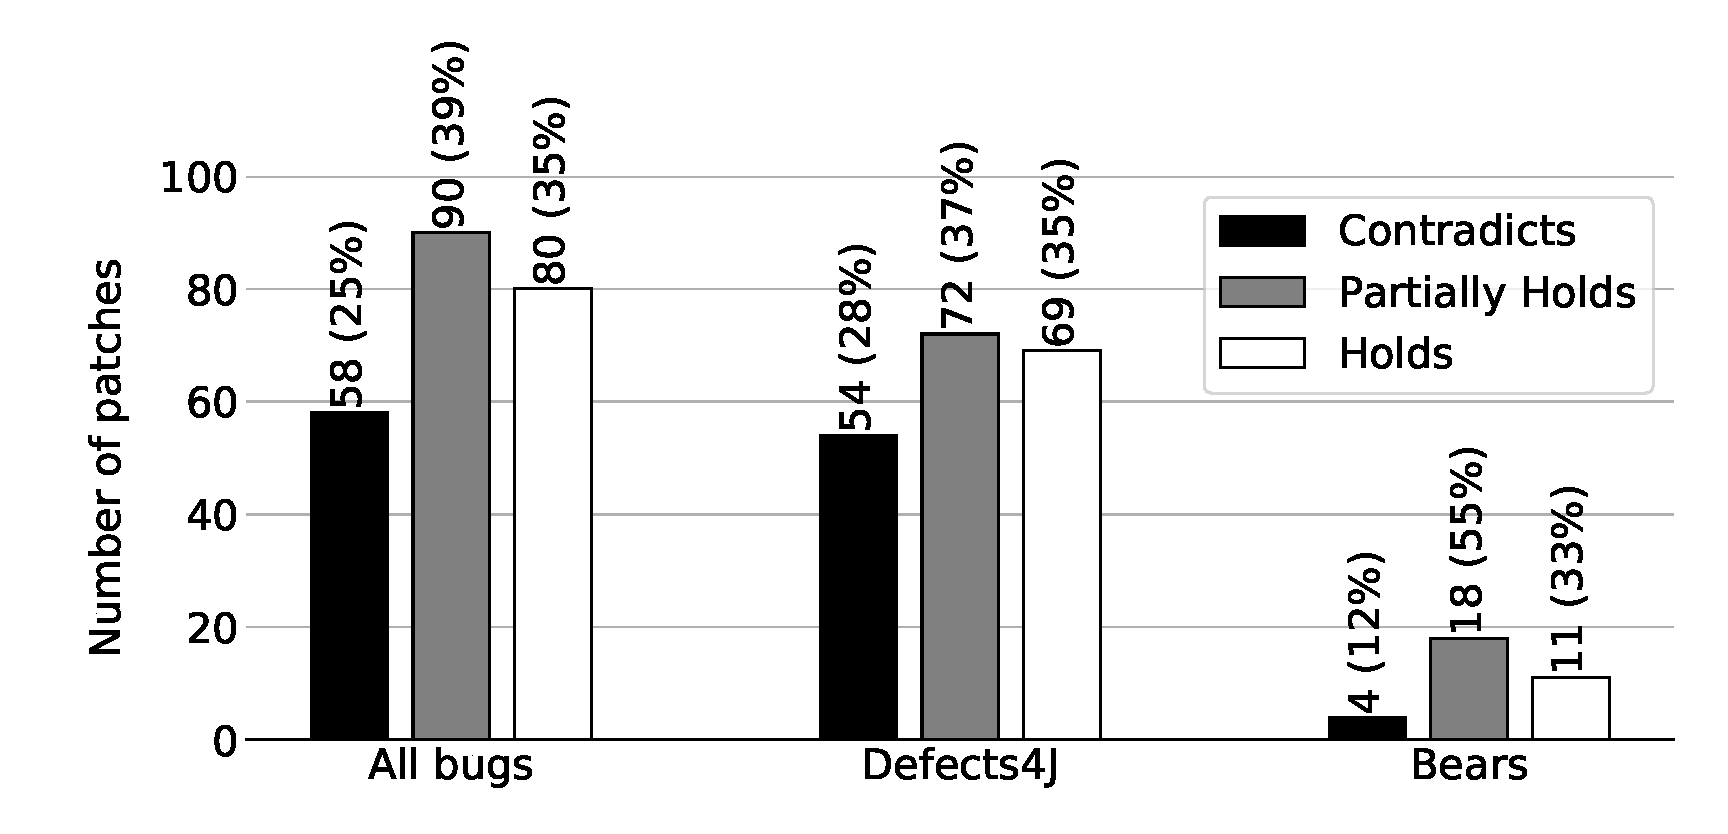
\includegraphics[width=\linewidth]{img/coverage_hist_all.pdf}
	\caption{\small Localization categories for multi-location bugs with multiple failing
      tests. The categories are relatively 
      evenly populated, with a slightly higher proportion of bugs in
      \emph{partially holds}. The datasets demonstrate different distributions.}
	\label{fig:coverage-all}
\end{figure}

\subsection{Results}
 \label{sec:cov_patterns}

\paragraph{Distribution of Localization Categories}
The first group of bars in Figure~\ref{fig:coverage-all} shows results for the overall distribution 
of localization categories, 
answering RQ2. 
For a 27\% bugs, none of the patch lines were executed by all failing tests as they were 
categorized as \emph{contradicts}.  A slightly larger proportion of bugs, 34\%, were classified 
as 
\emph{holds}, indicating that all failing tests executed the same patch lines.
In addition, another 40\% were classified as \emph{partially holds}.

Note, however, that the behavior varies considerably by dataset, as shown in the second and 
third groups of bars in Figure \ref{fig:coverage-all}. In particular, \bears has fewer bugs in 
\emph{contradicts} and more bugs in \emph{partially holds}.
This difference is statistically significant, with $p = 0.032$ (Fisher's exact test).
We hypothesize that this may be due to differences in how the two  
datasets were selected and constructed:
The Defects4J dataset specifically enforces a requirement that the patches in the 
dataset be isolated, i.e., not containing any refactorings or new features.
The authors both saught bugs that met this requirement, in manually isolated others~\cite{defects4j}. By contrast, the 
bugs in 
\bears bugs are scraped directly from continuous integration systems, and the 
only requirements for inclusion is that the bug must be reproducible and that
the patch must be written by a human~\cite{bears}. 
%In addition, Bears was designed to be evolvable 
%and relatively easily expanded as a dataset, which is at odds with manual inspection and isolation of 
%bugs~\cite{bears}.
%Given that these two datasets were designed with different values and demonstrate very 
%different behavior, 
These findings highlight the importance of diverse datasets
in APR evaluations. 

Out of the 124 bugs we checked, ten bugs had differing localization categories when 
classified based on coverage of patch lines vs. coverage of patch locations. All ten of these 
bugs 
were classified as \emph{partially holds} when classified by line coverage, but were classified as 
\emph{holds} when classifying by patch coverage, indicating that all the failing tests were 
executing different paths within the same patch locations. \todo{Is this discussion confusingly 
worded? Because patch locations refer to the patch chunk, made up of one or more lines of 
code.}

Overall, we cannot assume that the failing tests in multi-location repairs will execute all 
faulty locations -- in fact our results suggests that assumption only holds 32\% of the time. 
This suggests that off-the-shelf SBFL techniques may not be
well-suited to guiding APR techniques when addressing more than half of
real-world multi-location bugs. \todo{I think it's OK, actually.
Maybe ``are not'' can change into ``may not be,'' to soften a little bit. What
do you think of this version?}

\begin{figure}
	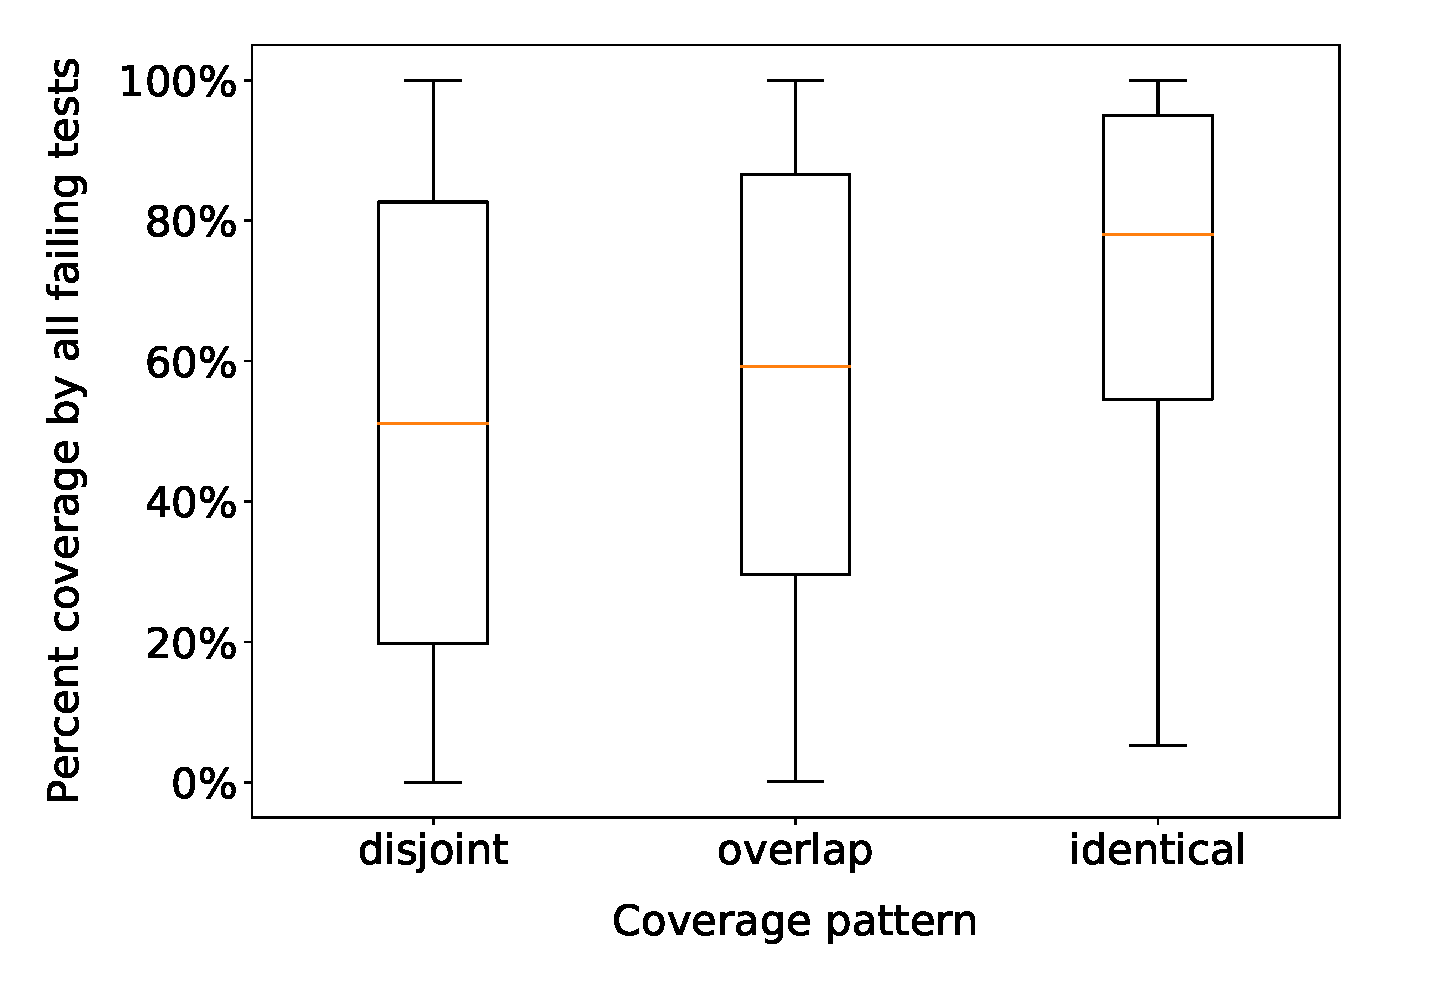
\includegraphics[width=\linewidth,left]{img/coverage-buggy.pdf}
	\caption{\small	\label{fig:coverage-buggy} Distribution of bugs based percentage of lines 
	executed by all failing tests, measuring the degree to which failing tests execute the same 
	code. The coverage distributions for the \emph{contradicts} and \emph{partially holds} are more or 
	less uniformly distributed. The coverage
	distribution for the \emph{holds} category skews measurable higher. 
      } %Thus, there seems to be little correlation between 
%	localization categories and whether failing tests all execute the same code in the buggy 
%	program.}
% CLG sez: I know I asked for takeaways in captions but (1) I'm not sure what
% this last one means and (2) I think it contradicts what we say in text, so I
% just cut it for space, it's fine. 
\end{figure}

\paragraph{Generalization of localization categories}
%<<<<<<< Updated upstream
Figure \ref{fig:coverage-buggy} plots localization category based on the
percentage of lines executed by all failing tests. 
%
The distributions of bugs in \emph{contradicts} (and to a lesser extent, bugs in \emph{partially 
holds}) are 
distributed apparently uniformly across 0\% to 100\% line coverage. This indicates that \emph{contradicts} 
bugs are 
not more/less likely to have failing tests that cover the same or different parts of the code 
base.
% JL: I agree that this is too confusing, cutting for now.
%% \footnote{Note that a bug categorized as \emph{contradicts} can be scored 100\% as the 
%% patch can introduce if statements that change the control flow and cause all failing tests to 
%% eventaully execute all different parts of the patch.\todo{I think this point may
%%   be too pedantic/confusing to be necessary, but let's try it in a footnote.}}
%
We qualitatively observe that bugs in \emph{holds} are more likely to have 
failing tests that execute the same lines of code, as we might expect. However, this is not 
definitive, as the failing tests in \emph{holds} bugs covered anywhere between 
5\% to 100\% of the same lines.

These observations are confirmed quantitatively: There were no statistically significant 
differences between the distribution for \emph{contradicts} and \emph{partially holds}. 
However, the distribution for \emph{holds} showed statistically significant differences with 
\emph{partially holds} ($p = 0.006$)  and \emph{contradicts} ($p < 0.001$).

In conclusion, 
we are not able to solely rely on degree to which failing tests cover the buggy 
code to always accurately classify bugs to their localization category.
However, \emph{holds} bugs tend to have failing tests that cover more of the 
same code than the failing tests of other bugs, indicating 
there may be ways we can augment this statistic to determine whether bugs would eventually 
be classified as \emph{holds}, which is 
especially notable since these bugs uphold our assumption and are accordingly more likely to 
succeed with SBFL.
 
\section{Mutation Operators and Fix Code}
\label{sec:mutops}

APR techniques vary in the types of
mutation operators they consider, how they select between them, and how they
select new fix code to instantiate them. 
%  For example, a na{\"i}ve
% approach with only \texttt{insert}, \texttt{replace}, and \texttt{delete}
% operators must choose between them at a location and, in the case of
% \texttt{insert} and \texttt{replace}, choose code to insert/replace at that
% location.  
%
%The few techniques that handle or at least enable multi-edit patches vary in their
%handling of mutation operator selection and instantiation.  
At one extreme, semantics-based repair~\cite{s3,angelix} can represent dependent edits between multiple
locations via as a conjunction of multiple simultaneous constraints; at the other, 
search-based or
evolutionary techniques~\cite{genprog,par} typically mutation
operators independently. 
% That is, a modification in one location does not
%inform the selection of a modifications to apply in a second location; instead,
%the heuristic search is trusted to 
The search space increases combinatorially, however, rendering
the chances of finding multi-edit repairs~\cite{ae,long-search-spaces}. Accordingly, heuristic multi-location
techniques~\cite{saha2019harnessing} make assumptions about the 
shape of the search space, 
targeting in particular bugs that can be repaired by multiple syntactically similar pieces of
code.

Note that the types of edits generally included in human patches has been
studied~\cite{examples}.  Here, we are especially
concerned about the 
\emph{relationships} between multiple edits, because such relationships have
key implications for how edits should be designed, selected, and instantiated 
in multi-location repair. 

\subsection{Dependencies}

One of the dimensions of the relationship between multi-location patches is potential
\emph{dependency} between the edits, because edit dependency can and should
inform how those edits are selected and applied (i.e., consider the difference
between a patch that applies the same edit in four places, and one that
applies four control-dependent
modifications).  Specifically, we ask:
\rqorinsight{4}{How prevalent and hard to construct are
patches with intra-patch dependencies?}


\paragraph{Methodology}
We consider a patch to contain \emph{dependent edits} if there exist 
control or data dependencies between added, deleted, or modified statements.
Since we analyze dependent statements, we broaden the scope of multi-location patches to 
include all patches containing at least two added, removed, or modified lines, 
again ignoring edits to comments, whitespace, or imports.
We denote such patches as \emph{multi-line patches}.
This expanded dataset contains 659 Defects4J v2 and 151 \bears 
multi-line patches.
% We explicitly got rid of Table 1 stats on multi-line 
% patches for ESEC/FSE. We did so since we didn't wish to divert attention 
% from multi-location patches during our discussion of the datasets in Sec 2.
% Dependency analysis is the only experiment that analyzes patches at the
% edit granularity of lines, rather than locations.
For practical performance and scalability reasons, 
we perform intraprocedural analysis. We added two heuristics for
interprocedural/field sensitive
information, namely assuming (1) that any invocations of a getter
method  \texttt{Class.getX()} reads \texttt{Class.X}, and (2) any invocation of 
 \texttt{Class.setX()} writes to  \texttt{Class.X}.
%
% We treat all method call statements as dependent on all variables
%passed as arguments. 
% CLG thinks is is just correct treatment of variables passed to method calls
While unsound, these heuristics derive from common Java
practices.
%We use these heuristics to estimate interprocedural 
%dataflow while retaining the scalability of intraprocedural analysis.
%We provide our dependency analyzer in our replication package.

We estimate the difficulty of auto-constructing edit-dependent patches 
by examining whether APR techniques have successfully patched the
bug in question. We use APR success data from 
RepairThemAll~\cite{durieux-repair-them-all}, an experiment 
running 11 APR tools on 5 benchmarks, including Defects4J v1
( a subset of Defects4J v2) and \bears.

\paragraph{Results}

\begin{table}
{\begin{center}
    \begin{tabular}{lrrrrrr}
        \toprule
        &\multicolumn{3}{c}{Without Dependent Edits} & \multicolumn{3}{c}{With Dependent Edits} \\
        Result& \multicolumn{1}{c}{Defects4J} & \multicolumn{1}{c}{\bears} & \multicolumn{1}{c}{Both} & \multicolumn{1}{c}{Defects4J} & \multicolumn{1}{c}{\bears} & \multicolumn{1}{c}{Both} \\
        \midrule
        Success & 96 & 7 & 103 & 43 & 9 &  52 \\
        Failure & 73 & 49 & 122 & 93 & 86 & 179\\
        \midrule
        Total  & 169 & 56 & 225 & 136 & 95 & 231\\
        \bottomrule
    \end{tabular}
 \end{center}
}	\caption{\small APR performance on bugs with and without intra-patch 
      dependencies, from RepairThemAll~\cite{durieux-repair-them-all}.%\protect\footnotemark
      \ \emph{Success} means that at least one of 11 APR tools found a patch; 
      \emph{Failure} means that no tool did.  APR tools found repairs 46\%
      (103/225) of the time for bugs with dependency-free human patches, but only
      23\% (52/231) of the time when a patch contained dependencies.}
	\label{tab:dependency-repair-contingency-table}
\end{table}
%\footnotetext{RepairThemAll provides results for Defects4J v1.}

Table~\ref{tab:dependency-repair-contingency-table}
shows frequencies of multi-line patches with respect to edit dependence 
and whether an APR tool successfully repaired the bug.
Our data substantiates prior research~\cite{zhong2015}:
45\% of the multi-location patches we study exhibit intra-patch dependencies. 
Importantly, 
we also find the presence of edit dependencies is correlated with lower rates of
APR tool success. 
Using a $\chi^2$ test, we find a statistically significant relationship ($p < 0.001$)
between APR success and intra-patch dependencies.
This result 
suggests that such dependencies indeed 
add complexity to the repair search in a way that challenges the state-of-the-art.
Dependent edits, however, may 
be an opportunity to constrain the search space by creating constraints between 
otherwise independent mutations.  There is an opportunity to profit from edit 
dependencies to repair a large class of difficult bugs.


\subsection{Cloned code}
\label{sec:clones}

\subsubsection{Occurrences of cloned code}

A patch composed of multiple, dependent edits constitutes one
extreme. At the other extreme lies patches that apply the same modification in several locations. 
Previous techniques have targeted exectly these types of
bugs~\cite{wang2018,saha2019harnessing}.  We evaluate how often this relationship applies to
multi-location bugs, and thus the usefulness of techniques that assume it:

\rqorinsight{5}{How often do clones occur in multi-location patches?}

%Possible intuition: if we can find some kind of correlation between fault localization results
%and code clones, then if some APR research decided to follow Wang et al's suggestion and
%include "repeat same edits at multiple location" operator, then our results may advise
%the APR to be more likely to apply the repeat edit operator when the fault localization
%result matches specific patterns.

%\paragraph{Methodology}
Our dataset includes all 216 multi-location bugs with 6 or fewer modified
locations (to reduce the analysis burden). We determine the existence of code 
clones through manual inspection.
%
% We cross validate our list of bugs with clones with results from previous work proposing and 
%evaluating an APR tool named Hercules~\cite{saha2019harnessing}. Hercules is a generate and 
%validate approach that could also exploit similar code locations to generate patches with code 
%clones. It was evaluated with the bugs in Defects4J version 1, which consists of 395 total bugs 
%and 187 multi-location bugs. 
%

Since we are studying code clones in patches, the same line of code could be inserted, deleted or modified, and conventional categorization of code clones into Type I,II,III,IV \cite{convcodeclone} does not apply to code modifications. Therefore, we devised our own standard of categorizing code clones in modifications as follows:
\begin{enumerate}
\item Same: The modifications at two locations are alpha-equivalent (i.e., the two locations are identical or would be
identical if we substitute all occurrences of a variable in one location with
another same-type variable). In studies on code clone detection, these are
referred to as Type-1 (if there are no changes) and Type-2 (if identifiers are
renamed) clones~\cite{kclone}.
\item Near-same: The edits at two locations are almost alpha-equivalent and
  differ by at most one constant or arithmetic operator,
or replacement of one constant with a variable.
\item Composite: The patch at one location is exactly copied and contained within the patch at 
the 
second location (the second location  has additional lines).
\item Move: One location is an insertion of 
code deleted from the other location. 
\end{enumerate}

%\paragraph{Results}
\begin{table}
{\begin{center}
\begin{tabular} {lrrrrrr}
\toprule
&&\multicolumn{2}{c}{Dataset} &\multicolumn{3}{c}{Locality}\\
& Total & Defects4J & \bears & Method & Class & Neither\\
\midrule
Same      &  80 &  71 & 9 & 35 & 33 & 12 \\
Near-same   &  25 &  23 & 2 & 12 &  8 &  5 \\
Composite &  12 &  11 & 1 &  4 &  8 &  0 \\
Move      &  12 &  11 & 1 &  9 &  1 &  2 \\
\midrule
Any       & 121 & 108 & 13\\
Total     & 372 & 308 & 64\\
\bottomrule
\end{tabular}
\end{center}
}
\caption{Code clone incidence, type, and location in our dataset. \emph{Same}, \emph{Near-same},
  \emph{Composite} and \emph{Move} are defined in Section~\ref{sec:clones}.
  \emph{Any} indicates any type of clone; note that some patches can
  contain clones from multiple categories. \emph{Locality} indicates
  the relative locations of clones in a patch (same method, class, or neither). 32.5\% of multi-location bugs
  in our dataset contain some form of cloning. }
\label{tab:clones}
\end{table}

Table~\ref{tab:clones} shows that 121 of 372 multi-location bugs
(32.5\%) included at least one type of cloning,
indicating a significant prevalence of code clones in multi-location human
patches.
%\footnote{Note that ``Any'' may not sum the previous rows because
%bugs can contain multiple pairs of code clones belonging to different
%categories.}
%
Moreover, close to half of code clones are in the same method, while less than
15\% of the cloning occurs across classes. Finally, 80 of 129 (62\%) of clones
fall in the ``same'' category, corresponding to alpha-equivalent code cloning.
These results suggest that when applying clones in program repair, 
most clones should be applied within the same class or the same method, and
in most cases a technique that only generates alpha-equivalent code clones should suffice.

% code clones <-> hercules data
% idk how what the conclusion from this information is so I'm just gonna put numbers in
% Hercules successfully repaired 15 multi-location bugs in their dataset. We found 56 
%multi-location bugs with clones. 14 of the bugs that Hercules successfully repaired were among 
%the bugs with code clones we found. The remaining bug that Hercules successfully repaired 
%was 
%a bug whose patch required 6 or more locations, and in going back, the human patch also 
%contained code clones. 
\subsubsection{Relationships between localization and clones}
Intuitively, we expect that bugs  \emph{contradicts} localization, where none of the patch is 
covered by all failing tests, are more likely to correspond to patches where
similar fix code is applied at multiple separately tested locations. If 
true, this suggests that fault localization information can help 
predict the utility of code clone-based APR mutation a priori. We ask:

\rqorinsight{6}{Does the existence of code clones in human patches correlate with specific 
localization patterns?}

% CLG sez: nice and clear, but derivable from first principles, and we have a
% length problem.
%By contrast, \emph{holds} bugs, where all failing tests execute 
%the same patch lines, may have
%more interrelated parts that are not merely the same statements copied to
%multiple locations.
%
We focus on the multi-test and multi-location bugs used in the coverage 
experiment (Section~\ref{secFL}, and exclude bugs with more than 6 faulty locations, leaving 191 bugs.

\begin{table}
  {\begin{center}
      \begin{tabular} {lrrrr}
        \toprule
        & Contradicts & Partially Holds & Holds & Total \\
        \midrule
        Clone & 26 & 12 & 11 &  49 \\
        No Clone  & 24 & 56 & 62 & 142 \\
        \midrule
        Total     & 50 & 68 & 73 & 191 \\
        \bottomrule
      \end{tabular}
    \end{center}
  }

  \caption{\small Multi-location and multi-test bugs classified by localization
    category (Section~\ref{secFL}) and patch clones. The category distribution
    is skewed toward \emph{contradicts} when patches contain code clones.}
  \label{tab:cov_clones}
\end{table}

Table~\ref{tab:cov_clones} shows the incidence of patch code clones among the three 
localization categories identified in Section \ref{secFL}. 
Out of 50 \emph{contradicts} bugs, 52\% (26/50) have clones; only 
18\% (12/68) and 15\% (11/73)
\emph{partially holds} and \emph{holds} bugs respectively contain clones.
A \emph{contradicts} bug is more likely to contain clones in its
human patch than bugs with other localization  ($p < 0.001$, by a $\chi^2$ test).. 
This suggests a heuristic for when to try a clone-based repair technique: if there
appears to be less coverage overlap between multiple failing tests, it is
possible that, if multi-location, 
applying the same edits at multiple locations~\cite{saha2019harnessing} may be
more likely to succeed. On the flip
side, however, these results also suggest that SBFL may not be well-suited to
guiding such techniques: 
53\% (26/49) of clone-containing patches exhibit \emph{contradicts}
localization, compared to 17\% (24/142) of non-clones. This suggests that clone
edits  are more likely to contradict SBFL's core assumptions
on fault coverage.  This motivates novel fault localization analyses for
clone-oriented techniques.   We
leave a concrete investigation of these possibilities to future work.  

% We also find that 
% Thus, clone edits are more likely to contradict SBFL's core assumptions
% on fault coverage, which suggests that clones are often contextually 
% \emph{different} enough to be not visible to all failing tests.
% Clone-oriented techniques such as Hercules~\cite{saha2019harnessing} may benefit
% from a non-SBFL technique.

\section{Test case-based validation}
\label{sec:tests}

Dynamic program repair typically uses test cases to validate patch plausibility. 
%, and tests
%are often used as a proxy for a full correctness specification. Tests are
%imperfect for this task, and virtually all APR techniques can \emph{overfit} to
%them~\cite{Smith15fse}, but they remain accessible and widely-used in practice.
%patches that satisfy the provided tests, but do not generalize to the
%higher-level specification~\cite{Smith15fse}.  
%
%Indeed, not all edits in a human patch are always necessary to pass all tests. This could be
%due to a human patch including refactoring or other changes that does not actually
%change code behavior~\cite{api-refactoring, tangledchanges}, or it could be a sign that the test
%suite is inadequate.  
Test case quality is a pressing problem in this context in
general~\cite{Smith15fse}, but perhaps especially in search-based approaches,
where tests typically inform the fitness
function. Here, ideally, test cases could usefully identify partial
solutions~\cite{better-fitness}, 
though whether tests are suitable for this purpose is a matter of
debate~\cite{ae,rsrepair}.  Sometimes, tests perform no differently on partial
repairs than they do on the original program~\cite{chris-thesis,
  source-code-checkpoint}; they have also been observed to perform
worse~\cite{gecco09}.  
%
We study this question in a principled fashion to characterize whether or how
tests can support multi-location patch construction.  That is, if we apply only one of
several of the edits in this patch to the buggy program, is the result
identifiable as ``closer'' to the full repair? Alternatively:

\rqorinsight{7}{How well do test case based validation methods identify partial repairs?}

If tests can in general identify partial repairs, this suggests the feasibility
of techniques that construct multi-location repairs by identifying/composing
partial repairs.

% CLG: ...can we get away without mentioning granularity here? Let's find out....
% Moreover, unit test performance can be measured in different granularity levels. 
% We would like to compare the performance of the fitness functions at identifying 
% partial repairs at different granularity levels.


\subsection{Methodology}
\label{sec:partial-repair-methodology}

In this experiment, we effectively apply all partial repairs for
a subset of multi-location bugs, and
evaluate how well the partially-patched programs perform 
as compared to both the original and the fully-patched versions. 

\subsubsection{Partial Repairs and Bug Selection}
We apply each non-empty subset of all location-level edits for a given bug to
its buggy program.  To minimize semantically invalid partial repairs, we \emph{always}
include edits that add import statements, helper methods/classes, or variable declarations
in a partial patch. 
For example, if a 3-edit patch contains a declaration of new variable
\texttt{var} at one location that is used at a second location, but not a third,
we include the first edit in all partial patches.  Note that this can reduce the total
number of partial patches per patch, and we eliminate
human patches that contain only 
one edit location after this preprocessing step. 

Due to the exponential growth of partial patches with respect to overall patch size,
we evaluate multi-location bugs with
between two and six edits, excluding Closure, which uses a
non-standard test harness. 
Overall, we evaluated 1884 Defects4J and 596 \bears partial repairs,
of 240 Defects4J and 74 \bears bugs.

\subsubsection{Test Granularity}

The standard use case for JUnit runs
an entire test \emph{class}, which ``passes'' if all test \emph{methods} in
that class also pass.  However, for the purposes of identifying partial repairs,
we can evaluate partial correctness at both the \emph{class-level} and
\emph{method-level} (a program that passes more methods is more
correct).
We also introduce and consider \emph{assertion-level} granularity, looking
roughly at how many assertions \emph{within} a method fail.  We define this as follows:
let $A(M)$ be the set of all \texttt{assert}
statements in a test method $M$. 
When $M$ is run, if an assertion failed, the failure is recorded and the method 
continues to run.  When the method completes, for each
$a\in A(M)$, let $b(a)$ be 1 if $a$ never failed once during execution,
and 0 otherwise. We define the \emph{assertion score} as
$AS(M)=\frac{\Sigma_{a\in A(M)}b(a)}{|A(M)|}$. If $M$ failed to run to completion 
due to timeouts or unrelated exceptions, then
$AS(M)=0$. Thus by definition, $AS(M)=1$ if $M$ passes. If a program passed more 
assertions in $M$, there should be an increase in $AS(M)$.


\subsection{Results}

\paragraph{Minimality} Our first immediate takeaway is that not all edits
in a human patch are always necessary to pass all tests~\cite{api-refactoring,
  tangledchanges}:
this is true for 41.3\%  (99 out of 240) of Defects4J and 52.7\% (39 out of 74) of
\bears bugs. 
The relatively high proportion of Defects4J patches that are not 1-minimal is
somewhat surprising, as Defects4J maintainers manually minimize patches to exclude
changes deemed unrelated to the bugs in question~\cite{documentation-maybe}.
This suggests that the test suites are weak proxies for total correctness.
\bears patches are not minimized, which likely explains
their higher percentage of non-minimality (52.7\%) (the difference between the two datasets is statistically
significant, $p < 0.001$, via a 
$\chi^2$ test).

\looseness-1
We compute results for RQ7 using the 1-minimal set of human edits
with respect to the unit tests as the ``full'' patch.
We do this for parsimony: including
unminimized edits introduces noise without materially changing
results.  And, from the point of view of an APR tool, only
minimal edits are identifiable or ``visible'' via test case behavior. 
We exclude bugs
minimized to a single edit, leaving
942 Defects4J and 232 \bears partial repairs, from
165 Defects4J and 44 \bears bugs.  

% We therefore present our results for RQ7 in two ways:
% treating the provided human patch as the full repair
% (Unminimized), and considering only the 1-minimal set of edits in the
% human patch with respect to the unit tests (Minimized).

\paragraph{Partial repair identification} Our overall goal is to identify how many partial repairs pass more test than the
original buggy program  (\emph{positive}), the  same number of tests as the
original buggy code (\emph{neutral}) or fewer tests than the buggy code
(\emph{negative}).  However, 
since each bug can have a different 
number of partial repairs, we
scale the partial repair results to give each bug equal weight.
That is, for a bug with $n$ partial repairs, each edit has weight 
$\frac{1}{n}$.\footnote{We exclude partial
repairs that do not compile from the count, e.g., by throwing errors like ``missing return statement.''}


%\begin{table}
%{\begin{center}
%\begin{tabular}{ll|rr|rr|rr}
%\toprule
%\multicolumn{2}{c}{}&\multicolumn{2}{c}{Defects4J} & \multicolumn{2}{c}{\bears} &\multicolumn{2}{c}{Combined}  \\
%\multicolumn{2}{c}{Minimized?} & \multicolumn{1}{c}{No} & \multicolumn{1}{c}{Yes} & \multicolumn{1}{c}{No} & \multicolumn{1}{c}{Yes} & \multicolumn{1}{c}{No} & \multicolumn{1}{c}{Yes}  \\
%\midrule
%\multirow{3}{*}{Positive} & Class & 25.95\% & 12.77\% & 23.87\% & 9.22\% & 25.46\% & 12.02\% \\
% & Method & 40.82\% & 34.58\% & 28.41\% & 18.23\% & 37.90\% & 31.14\% \\
% & Assertion & 44.49\% & 39.93\% & 28.68\% & 18.69\% & 40.76\% & 35.46\% \\ 
%\midrule
%\multirow{3}{*}{Neutral} & Class & 59.56\% & 68.30\% & 58.97\% & 73.31\% & 59.42\% & 69.35\% \\
% & Method & 39.62\% & 40.05\% & 53.08\% & 64.30\% & 39.93\% & 40.83\% \\
% & Assertion & 33.73\% & 31.52\% & 49.52\% &  59.60\% & 37.45\% & 37.43\% \\ 
%\midrule
%\multirow{3}{*}{Negative} & Class & 9.30\% & 11.57\% & 8.78\% & 13.30\% & 9.18\% & 12.16\% \\
% & Method & 13.51\% & 17.16\% & 10.13\% & 13.30\% & 12.71\% & 16.35\% \\
% & Assertion & 15.37\% & 19.80\% & 12.75\% &  16.41\% & 14.75\% & 19.09\% \\ 
%\bottomrule
%\end{tabular}
%\end{center}}
%\caption{Weighed percent of partial repairs exhibiting a {\normalfont Positive}, {\normalfont Neutral},
%	or {\normalfont Negative} change in test passage, measured at different levels of granularity
%	and with both minimized and unminimized patches.\todo{big ole todo: cut
%          the ``unminimized'' results and turn this into a histogram; see my bad
%          sketch in Slack.}}
%\label{yiweitable}
%\vspace{-0.5in}
%\end{table}

\begin{figure*}
        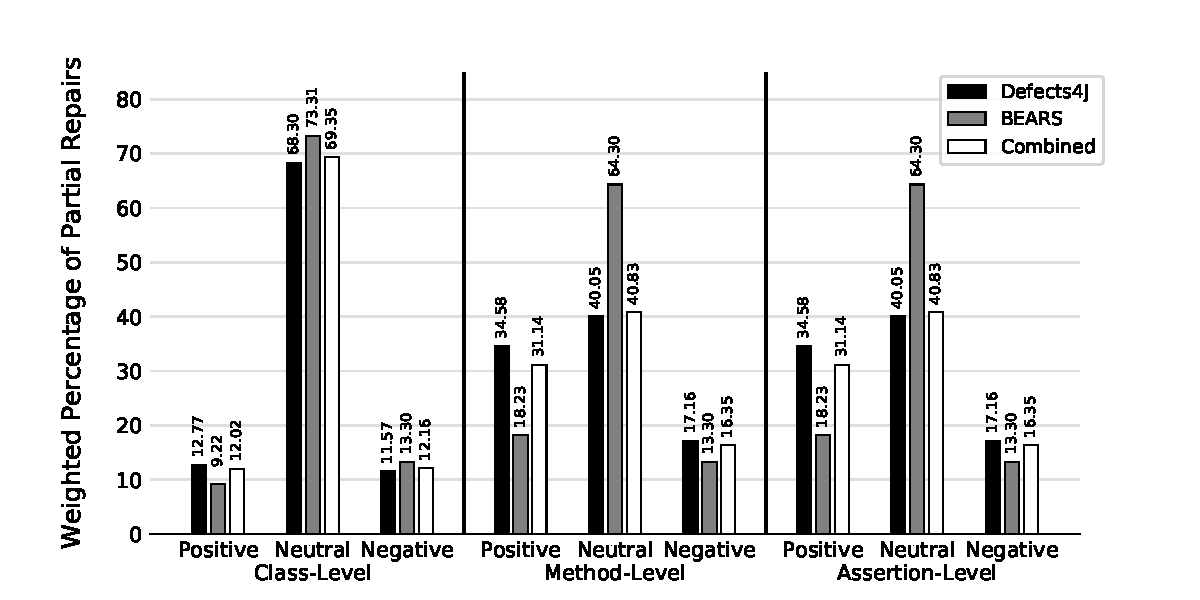
\includegraphics[width=\textwidth]{img/weighted_percent.pdf}
        \caption{Weighted percent of partial repairs exhibiting a {\normalfont
            Positive}, {\normalfont Neutral}, or {\normalfont Negative} change
          measured at varying levels of granularity. As granularity increases
          the negative partial repair rate remains low, while the positive
          repair rate rises significantly.}
        \label{fig:fitness}
\end{figure*}


Figure~\ref{fig:fitness} shows results.
Assertion level granularity correctively positively identifies
39.93\% of the partial repairs in Defects4J
and 18.69\% of the partial repairs in \bears.
Only 31.52\% of Defects4J partial repairs and 
59.60\% 
of \bears partial repairs are neutral. Less than 20\% of bugs in both datasets
produce negative test case behavior.
Although the rate of positive and correct identification of partial repairs varies between datasets,
tests are not often adversarial towards partial repairs, contrary to anecdotal
observations in prior work~\cite{gecco09}.

\paragraph{Granularity} Finer granularity levels are better at identifying partial repairs positively,
but they also increase the chance of erroneously mis-identifying partial repairs.
Improvements between granularity levels vary across datasets --- the improvement 
in positively identified partial repairs between method and assertion level granularities
is negligible in \bears (0.46\%) but greater in Defects4J (5.35\%), while both had around 3\% 
increase in negatively identified partial repairs.
Moreover, evaluating patches at finer granularity levels can add overhead.
For example, assertion level granularity requires instrumenting JUnit with additional
logic to continue execution when assertions fail.
Such overhead lowers the number of
candidate patches that a G\&V tool can validate per unit time.
The choice of a granularity level is a balancing act with implications for
multiple axes of APR performance.


\begin{table}
  {\begin{center}
      \begin{tabular} {llrrrr}
        \toprule
        \multicolumn{2}{c}{Partial Repair} & Contradicts & Partially Holds & Holds & Total \\
        \midrule
        \multirow{2}{*}{Positive} & $\exists$  & 40 & 30 & 12 &  82 \\
                                  & $\nexists$ &  1 &  4 & 16 &  21 \\
        \midrule
        \multirow{2}{*}{Negative} & $\exists$  &  2 &  8 & 16 &  26 \\
                                  & $\nexists$ & 39 & 26 & 12 &  77 \\
        \midrule
        Total                     &            & 41 & 34 & 28 & 103 \\
        \bottomrule
      \end{tabular}
    \end{center}
  }
  \caption{\small Multi-test bugs categorized by both localization pattern
    (Section \ref{secFL}) and existence of positively/negatively identified
    partial repairs. Bug patches with the \emph{holds} coverage pattern are
    statistically significantly more likely to exhibit negative partial
    repairs.  \label{tab:cov_fitness}}
\end{table}

\paragraph{Relationship to fault localization} 
Finally, we assess the relationship between partial repair behavior and fault
localization/coverage pattern. Table~\ref{tab:cov_fitness} shows 
bugs with 2+ failing tests 
and 2--6 edit locations in the minimized patch, grouped by localization
categories (Section~\ref{secFL})
and the existence of positively/negatively
test-identified partial repairs at any granularity level.
In general, bugs with \emph{holds} localization (where failing tests execute
more similar locations) are less likely to have
positive partial repairs and more likely to have negative partial repairs (statistically significant,
$p < 0.001$ for both, via $\chi^2$ tests).
Thus, a \emph{holds} localization pattern correlates with an
\emph{adversarial} test-based fitness landscape,
and partial repairs may be harder to identify using tests for such bugs. 

These connections 
suggest that fault-revealing tests' patch coverage reflect the tests' ability
to detect components of a patch.
Recall that \emph{holds} localization means all failing tests execute 
the exact same set of patch lines, and \emph{contradicts} localization 
means no patch line is covered by all failing tests.
Intuitively, if a patch can be
assembled from two components \textbf{A} and \textbf{B}, two tests that both
fully cover \textbf{A} and \textbf{B} are less effective at assessing partial
correctness than two tests that only cover \textbf{A} and \textbf{B} separately.
Coverage thus influences the accuracy of tests as a judge of partial correctness.

In practice, we do not know patch coverage \emph{a priori}  
since we do not have a full patch yet. However, if we can infer the
likelihood of a bug belonging to the \emph{holds} category using existing 
fault localization (since \emph{holds} requires all failing tests to cover the 
entire patch), then we can relax judgements of partial correctness to 
preserve more partial repairs that might otherwise be rejected.

\section{Limitations}
\label{sec:limits}

\noindent\textbf{Coverage.}
We use JaCoCo to collect coverage, but it has some
limitations. It cannot analyze coverage for inserted
cases for \texttt{switch} statements, \texttt{else} statements, method
signatures, and other code constructs that are compiled away during the
transformation to bytecode. Since we focus on how the coverage of different
failing tests compared to each other, we posit that JaCoCo's coverage was a
sufficient approximation.

\vspace{1ex}
\noindent\textbf{Dependency analysis.}
We analyzed dependencies intraprocedurally with some interprocedural 
heuristics, which make assumptions derived from common Java practices.
These assumptions are not always true. We use heuristics to add some
approximated interprocedural data while retaining interprocedural 
analysis's scalability to large, real world software.

\vspace{1ex}
\noindent\textbf{Code clones.}
We examined code clones at the location level.  However, clones also occur at the
granularity of lines~\cite{JiaClones} or
subexpressions~\cite{microclones}. We classified clones into four
categories (Same, Near-same, Composite, Move), but other categorizations 
are possible.
%
We did not distinguish between the number
of edit locations in a particular set of clones. It is possible that a set of
clones contains two or more locations with similar edits, which we do not examine. 

\vspace{1ex}
\noindent\textbf{Partial repair construction.}
We constructed partial repairs by breaking up multi-location patches
into single-location edits.
In reality, most APR techniques mutate code at a finer granularity, so
these edits may not be representative.  Additionally, we only observe if test suites
can identify partial repairs. Perhaps our evaluated partial repairs
are outside of the search space of a
particular APR technique.
%Regardless of this limitation, this experiment provides valuable 
%insight into the challenge of automatically constructing
%multi-location patches.

\section{Related Work}
\label{sec:related}

\todo{Does this include related work since ESEC/FSE?  Quickly check out this
  year's ICSE, if nothing else.}
\todo{Also, this is long, but we can do a cutting pass when we're focusing on length.}
Recent empirical studies on fault localization find that 
SBFL is more effective than various other techniques, such as 
mutation-based fault localization~\cite{pearson2017evaluating, mut-analysis}, program 
slicing, predicate switching,  information retrieval, and other techniques. 
However, a 
technique that outperforms all of these can be created using machine learning to combine 
multiple fault localization techniques, implying that different techniques can 
localize different kinds of faults~\cite{zou2019empirical}. Most empirical 
studies on fault localization evaluate techniques by determining whether a 
technique can localize any faulty line. This usefully evaluates single line or single 
location faults, but not necessarily multi-location faults.

Golagha et. al~\cite{golagha2020can} analyzed the impact of 70 code metrics on SBFL, and built 
a machine learning model to predict the bugs that would succeed with SBFL. With regards to 
multi-location patches, the number of locations changed in the human 
patch was among the metrics they tested and was not found to be correlated to SBFL success. 
However, success was defined as ranking any faulty method in the top ten, which we argue is 
not adequate for localizing multi-location faults. 

Mutation testing contains parallels to program repair, as seen in G\&V
program repair~\cite{weimer2013leveraging} and fault 
localization techniques~\cite{metallaxis,muse,mbfl-survey}. 
There is recent work on higher order mutants, which is interested in finding 
certain combinations of mutants with particular behaviors. Higher order mutation testing 
shares similar difficulties with multi-location bugs, particularly due to 
exponential search space growth~\cite{long-search-spaces}. 
The current state of the art in finding specific classes of 
higher order mutants is using search based approaches; in particular, the best approach 
currently identified is a genetic search, which is reminiscent of program repair~\cite{homs, 
genprog}.

Qi et al.~\cite{patch-correctness} evaluated patches generated 
by three G\&V repair tools~\cite{genprog, ae, rsrepair}. 
The vast majority of generated patches were incorrect and equivalent to 
a single functionality deletion.  Patch \emph{overfitting} to the provided test
cases can be measured via the use of held-out test
suites~\cite{Smith15fse}, a technique that empirically validates the challenges of producing
high-quality repairs in response to a single test suite.   Later work found patch incorrectness to be 
also problematic in Defects4J~\cite{d4j-eval} and in semantics-based 
repair techniques~\cite{Le2018}.  We similarly find that test suites provide
imperfect semantic coverage over multi-location edits: many bugs can be fixed
with only a portion of a multi-location human patch.  We 
also find, however, that test cases can often identify partial patches. 

% I know I'm referring to the work by the authors' names,
% but I can't find a good way to refactor their names out without writing awkwardly.
% I would need to refactor all of the usages of "they" to remove their names.
Long and Rinard~\cite{long-search-spaces} studied
correct and incorrect plausible patches in the search spaces of SPR~\cite{spr} 
and Prophet~\cite{prophet}. They found incorrect plausible patches to outnumber 
correct patches by orders of magnitude. When they increased the search space 
by adding additional mutation operations, they found an increased number of 
correct patches, but APR tool performance might actually degrade due to a 
simultaneous increase in incorrect plausible patches and growth in search space.  
While we do not study this particular problem, 
we similarly seek to understand the 
massively larger search space of multi-location repair. 

A previous empirical study on real bug fixes~\cite{zhong2015} 
studied fault localization difficulty, bug fix complexity, necessary
mutations, relevance of API knowledge, and buggy file types
on more than 9000 real-world bugs.  
Both our paper and the previous study aim to provide useful guidance and insights for 
improving state-of-the-art APR techniques through empirical studies of bugs and bug fixes. 
Our study differs in that we focus on 
source code bugs patched by multiple edits in multiple locations. 
We draw insights in fault localization, fix mutations, and test-based 
patch evaluations. Additionally, we study the program repair 
benchmark datasets Defects4J 
and \bears; we believe that the program repair community would derive 
benefit from a study of APR benchmarks.

Wang et al.~\cite{wang2018} empirically studied multi-entity changes in bug patches 
(where each entity is a class, method or field). They queried
why and how often do patches have multi-entity changes, relationships 
between co-changed entities, and recurring patterns of multi-entity changes. 
By analyzing 2854 real-world bugs from four projects, they found that 66\%-76\% of
multi-entity fixes contain dependencies, 
and they identified three major recurring patterns that connects co-changed entities. 
They suggested a potential way to 
enhance APR by incorporating multi-entity changes. In contrast, we focus on bugs that
requires multiple edits to fix, where the edits may be in the same entity. In addition 
to reinforcing their earlier findings on intra-patch dependencies, we discover 
additional insights for enhancing APR in the axes of fault localization, 
fix mutations, and patch validation.

Hercules~\cite{saha2019harnessing} is an APR technique that takes 
advantage of fix code similarity to generalize a single repair edit into a 
patch consisting of multiple similar edits.
We discuss fix code similarity and insights on Hercules in 
Section~\ref{sec:clones}.

Prior work in program repair to use more search-guiding information 
during candidate patch evaluation 
include using program invariants~\cite{better-fitness, dinglyu}, 
intermediate program values~\cite{source-code-checkpoint}, 
and online mutation-based fault localization~\cite{mut-analysis}.
Some approaches require additional input, such as suspicious variables~\cite{source-code-checkpoint} 
or known patches for the bug under repair~\cite{better-fitness}, 
while others exhibit limited performance improvements~\cite{dinglyu, mut-analysis}.
We show the potential benefit of deriving more information from tests
with assertion level granularity.
Future work may explore more methods to mine information from tests 
beyond passage or failure.

Schulte et al.~\cite{schulte} found that 37\% of code mutations 
do not change test case passage and discussed potential applications 
of mutation robustness in proactive bug repair. 
Although our context differs --- they studied random mutations, 
we study changes associated with specific bug fixes --- we also find a 
non-trivial proportion of neutral edits in multi-location repairs.


\section{Takeaways and Conclusions}
\label{sec:takeaways}

Our findings demonstrate that bugs repaired with multi-location patches have
fundamental differences from bugs repaired with single-location patches. These
differences should be considered for designers of future APR techniques that
generate multi-location bug fixes. These are our key takeaways:

\todo{I kind of think this formatting is ugly, but I get the motivation.  Do
  these takeaways include the data/experiments added for ICSE 2021?  Anyway,
  I'll reread at the end.}
\begin{itemize}[wide, labelindent=0pt]
\item \textbf{Assumptions underlying spectrum-based fault
  localization do not always hold in multi-location bugs.}
In particular, the assumption that faulty locations
are executed more often by negative test cases was not true for a substantial
number of bugs in our study. In our study 40\% of bugs repaired with
multi-location patches and characterized by multiple failing tests had patch
locations that executed by some but not all tests; thus the assumption was only 
partially held.
Additionally, 27\% of
these patches had no patch location covered by all failing
tests, and thus contradicted the assumption.  
Patches with clones are especially likely (53\%) to contradict the assumption.
In these cases SBFL is unlikely to be the most 
appropriate choice for a
fault localization technique. This finding suggests that there is still progress
to be made in fault localization for automated repair.

In addition, bugs for which failing tests all execute the same faulty locations (i.e. bugs for 
which the assumption is true) are more likely to have failing tests that execute very similar 
parts of the program, indicating that there may be a way to identify these bugs.

\item \textbf{Patches with dependencies are common and harder to construct.}
We found that 45\% of human-written multi-location patches contained
intra-patch control and data dependencies. These patches are less likely to be
generated by a broad range of repair techniques. 
% Semantic APR can generate dependent code, and can sometimes even 
% account for constraints imposed by dependencies.
% Whether semantic APR techniques are any better at practically generating 
% dependent patches, however, is a data analysis task for the journal extension paper.
This points to an opportunity to exploit dependencies by
existing or new techniques to improve APR for this large class of hard-to-repair
bugs.

\item\textbf{Code clones are prevalent in multi-location patches.}
We found code clones in 32.5\% of bugs with multi-location
patches. This observation supports recent work that leverages code clones to
generate repairs~\cite{saha2019harnessing}.
We also found that clones are more likely to contradict SBFL's assumptions 
on coverage, which suggests both a heuristic for clone application and the
potential benefits of other fault localization paradigms.

\item\textbf{Correct partial repairs rarely cause more failing tests.}
Contrary to prior work~\cite{gecco09}, we found that test suites are infrequently
hostile to partial repairs. That is, partial application of a correct patch
usually does not increase the number of test case failures. This means that
generate and validate APR techniques can assemble correct patches from partial repairs.

\item\textbf{Patch coverage should be considered when determining the
  confidence of a test suite's assessment of partial correctness.}
Test cases are a more accurate metric of partial correctness when coverage
overlap of patch components is lower (the non-\emph{holds} localization cases).
We can reduce the possibility of overlapping coverage by decomposing tests into
smaller units, potentially by
refactoring~\cite{b-refactoring} or using a finer level of granularity for
measuring test suite success, such as the assertion level granularity proposed
in Section~\ref{sec:partial-repair-methodology}.

This also implies that class-level granularity validation has tradeoffs. Some
repair frameworks use class-level granularity for faster validation. This may
come at the cost of less accurate detection of partial patches. However, this
tradeoff may be worthwhile in Java, given the non-trivial challenges involved in
decomposing JUnit test classes into individual methods.

\item\textbf{Human patches are often not test-minimal.}
Many bugs do not need all patch locations to pass all tests,
offering further evidence of the incompleteness of test cases as a
proxy for correctness~\cite{patch-correctness} and the
presence of non-corrective changes (e.g., refactoring, enhancements)
in handwritten bug patches~\cite{api-refactoring, tangledchanges}.

\item\textbf{Techniques need to be evaluated on diverse benchmarks.}
Our two datasets, Defects4J and \bears, exhibited different characteristics.
These characteristics may explain why APR tools perform unevenly across
different benchmark datasets~\cite{durieux-repair-them-all}. Our findings
provide evidence reinforcing the call for the use of diverse benchmarks when
evaluating tools.
\end{itemize}

To date, most automated program repair techniques have been limited to bugs that
can be localized to and repaired at a single program location. However, we find
that 50\% of bugs in the Defects4J dataset and 61\% of bugs in the \bears dataset
were repaired by a human developer with multi-location patches. This motivated
our study on the possibility of extending current program repair work to
multi-location patches.

Our study's findings suggest deep implications for program repair targeting
multi-location patches, both in terms of the applicability of existing program
repair techniques and the design future repair techniques.  We hope that our
findings and insights inspire future work to advance the state of the art of APR
and take on difficult multi-location bugs.

\bibliographystyle{IEEEtran}
\bibliography{references}

\end{document}
\endinput
